\section{ВЕРИФИКАЦИЯ ОПТИМИЗИРОВАННОЙ ВЕРСИИ АЛГОРИТМА}

Рассмотрим СЛАУ с $\vb{b} = (1,1,1,1,1)^\mathrm{T}$ и матрицей
\begin{equation*}
    \vb{A} = 
    \begin{pmatrix}
        6&1&1&1&1 \\
        1&6&1&1&1 \\
        1&1&6&1&1 \\
        1&1&1&6&1 \\
        1&1&1&1&6 \\
    \end{pmatrix}.
\end{equation*}
На Рис. \ref{fig:screenshot} показан результат работы программы при числе процессов, равном 1 и 4. Программа выводит на экран транспонированный вектор решения $\vb{x}^T$.
\begin{figure}[htbp]
    \centering
    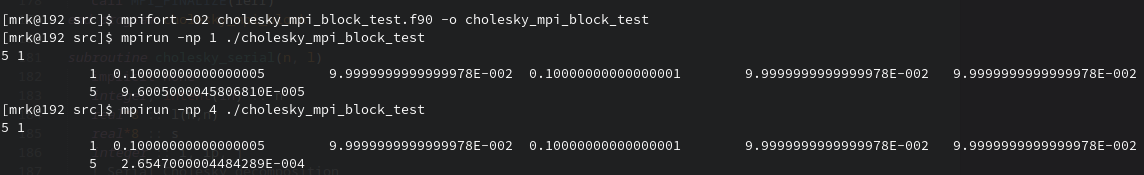
\includegraphics[width=\textwidth]{fig/screenshot.png}
    \caption{Результат работы алгоритма при одном потоке и при четырех потоках, на экран в первой строке выводится номер строки (в данном случае всегда 1) и сам транспонированный вектор решения $\vb{x}^T$, а на второй --- размер матрицы $n$ и время работы.}
    \label{fig:screenshot}
\end{figure}
Видно, что как при одном процессе, так и при двух процессах программа выдает правильный ответ $\vb{x}^T = (0.1,\,0.1,\,0.1,\,0.1,\,0.1)^T$ с машинной точностью.